%%%%%%%%%%%%%%%%%%%%%%%%%%%%%%%%%%%%%%%%%%%%%%%%%%%%%%%%%%%%%%%%%%%%%%%%%%%
%
% Template for a LaTex article in Slovak.
%
%%%%%%%%%%%%%%%%%%%%%%%%%%%%%%%%%%%%%%%%%%%%%%%%%%%%%%%%%%%%%%%%%%%%%%%%%%%

\documentclass{article}

\usepackage[utf8]{inputenc}
\usepackage[slovak]{babel}
\usepackage[document]{ragged2e}
\usepackage{amsmath}
\usepackage{siunitx}
\usepackage{multicol}
\usepackage{textcomp}
\usepackage{amsmath, amsthm, amsfonts}
\usepackage{graphicx}
\usepackage{url}
\usepackage{subcaption}
\usepackage{float}
% Theorems
%-----------------------------------------------------------------
\newtheorem{thm}{Theorem}[section]
\newtheorem{cor}[thm]{Corollary}
\newtheorem{lem}[thm]{Lemma}
\newtheorem{prop}[thm]{Proposition}
\theoremstyle{definition}
\newtheorem{defn}[thm]{Definition}
\theoremstyle{remark}
\newtheorem{rem}[thm]{Remark}

% Shortcuts.
% One can define new commands to shorten frequently used
% constructions. As an example, this defines the R and Z used
% for the real and integer numbers.
%-----------------------------------------------------------------
\def\RR{\mathbb{R}}
\def\ZZ{\mathbb{Z}}

% Similarly, one can define commands that take arguments. In this
% example we define a command for the absolute value.
% -----------------------------------------------------------------
\newcommand{\abs}[1]{\left\vert#1\right\vert}

% Operators
% New operators must defined as such to have them typeset
% correctly. As an example we define the Jacobian:
% -----------------------------------------------------------------
\DeclareMathOperator{\Jac}{Jac}

%-----------------------------------------------------------------
\title{Zadanie 4}
\author{Miroslav Kurka\\
  \small Dept. of Biophysics\\
  \small Pavol Jozef Šafárik University in Košice\\
  \small Slovakia 
}

\begin{document}
\maketitle


\section{Úloha}

Odhadnite hodnotu určitého integrálu
\begin{equation}
    \int_{0}^{1} \frac{\arcsin{x}}{x} dx = \frac{\pi}{2} * \ln{2} 
\end{equation}
pomocou MC integrovania. 



\textbf{a)} Graficky vykreslite váš MC odhad hodnoty integralu ako aj chyby s použitím
neskresleného odhadu štandardnej odchýlky. Pre generovanie postupnosti n uniformných náhodných čísel z intervalu [0,1]
použite príkaz rand(1,n).


\textbf{b)} Preveďte numerický experiment ako priamo merať štandardnú odchýlku MC odhadu. Za
týmto účelom, pre každé M odhadnite I Nseed-krát s použitím Nseed rôznych počiatočných
hodnôt, tzv. seed (pomocou príkazu rand("seed", x), kde x sú rôzne hodnoty)
generátora NČ (použite Nseed = 100). Vypočítajte štandardnú odchýlku $\sigma_M$ týchto Nseed
odhadov I1,I2 ... INseed
\begin{equation}
    \sigma_M = \sqrt{\frac{1}{N_{\text{seed}}} \sum_{i=1}^{N_{\text{seed}}} (I_i)^2 - \left(\frac{1}{N_{\text{seed}}} \sum_{i=1}^{N_{\text{seed}}} I_i\right)^2}
\end{equation}
    
Vykreslite vypočítané hodnoty $\log{\sigma_M}$ ako funkciu log10M pre $M = 10, 10^2, 10^3, 10^4 a 10^5$
spolu s jej neskresleným odhadom z úlohy a/. (sú si podobné?). Ak MC chyba klesá ako
$\sigma_M=\frac{C}{\sqrt{M}}$, kde C je štandardná odchýlka celej populácie (viď prednášky), potom
\begin{equation}
    \log{\sigma_M} = \log{C} - \frac{1}{2} \log{M}
\end{equation}

takže môžete fitovať dáta priamkou so smernicou -0.5. Odovzdajte program a graf.


\subsection{Teória}\label{sec:nothing}

Výpočet integralú pomocou MC metódy je založený na náhodnom výbere bodov z oblasti, ktorú chceme integrovať\cite{Zukovic}. V našom prípade je to oblasť $[0,1]$. Výpočet je založený na nasledujúcom vzorci:
\begin{equation}
    \int_{a}^{b} f(x) dx = (b-a) \frac{1}{N} \sum_{i=1}^{N} f(x_i)
\end{equation}
kde $x_i$ je náhodná premenná z oblasti $[a,b]$, $N$ je velkosť vzorky (počet náhodných bodov $x_i$). V našom prípade je to $[0,1]$. Výpočet je založený na tom, že náhodne vygenerované body z oblasti $[0,1]$ sú rovnomerne rozložené. Preto je možné použiť vzorec (4) na výpočet integrálu. 


\subsection{Výsledky}


\begin{figure}[H]
    \centering
    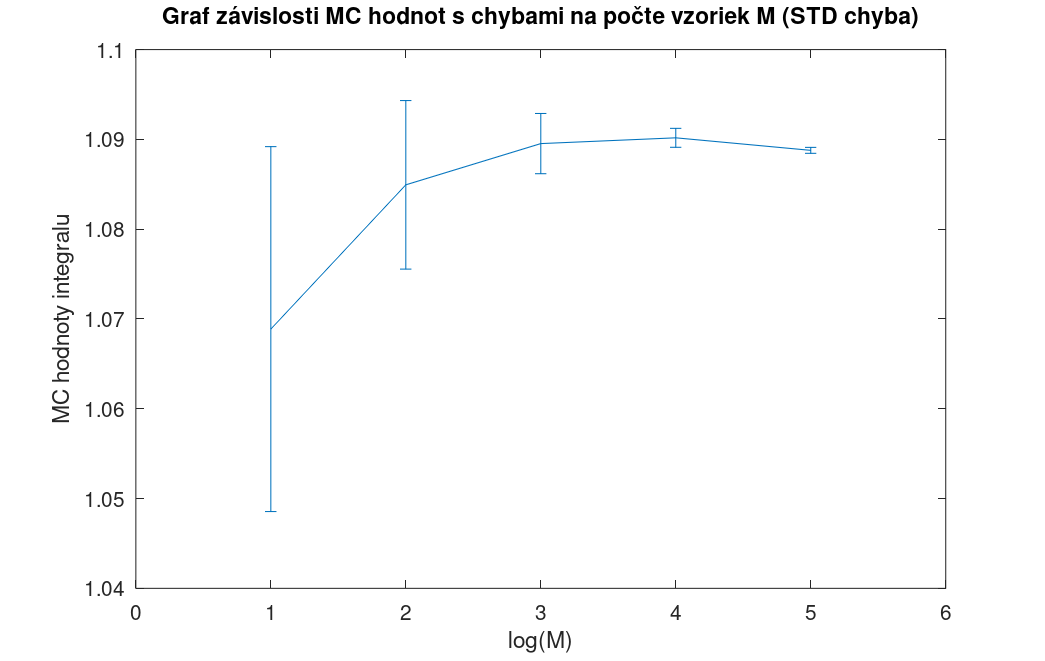
\includegraphics[width=1\textwidth]{hw4stdgraph.png}
    \caption{Riešenie integralu pre veľkosti vzoriek $M = 10, 10^2, 10^3, 10^4 a 10^5$ s neskresleným odhadom štandardnej odchýlky.}
    \label{fig:mc}
\end{figure}

Graf \ref{fig:mc} ukazuje hodnoty odhadu integralú z úlohy a) pre veľkosti vzoriek $M = 10, 10^2, 10^3, 10^4 a 10^5$ s neskresleným odhadom štandardnej odchýlky. Na osi x je logaritmus veľkosti vzorky M a na osi y je hodnota integralú. "Error bar" zobrazuje hodnotu štandardnej odchýlky.

\begin{figure}[H]
    \centering

    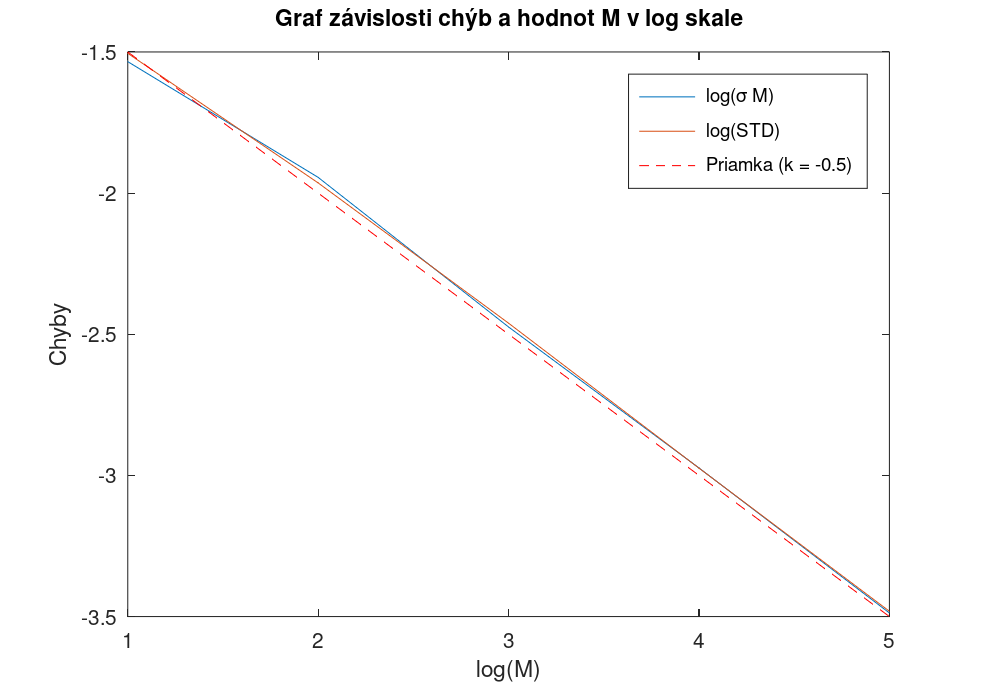
\includegraphics[width=1\textwidth]{hw4chyby.png}
    \caption{Chyba $\sigma_M$ v logaritmickej škále pre veľkosti vzoriek $M = 10, 10^2, 10^3, 10^4 a 10^5$ spolu s neskresleným odhadom (taktiež log škále) z úlohy \textbf{a)}.}
    \label{second}

\end{figure}

V Obr. \ref{second} sú vynesené hodnoty logaritmu odchýlky $\sigma_M$ ako funkcie logaritmu veľkosti vzorky M pre $M = 10, 10^2, 10^3, 10^4 a 10^5$ spolu s jej neskresleným odhadom z úlohy \textbf{a)}. Hodnoty sú následne fitované priamkou so sklonom -0.5.

\subsection{Záver a Diskusia}
V grafe \ref{fig:mc} je vidieť, že s vyššim počtom vzoriek M tj. nahodných bodov vyhodnotených sa odhad integrálu približuje reálnej hodnote integrálu $\frac{\pi}{2} * \ln{2}$. Taktiež je vidieť, že štandardná odchýlka sa znižuje s vyššim počtom vzoriek M.   



Graf \ref{second} zobrazuje neskresleného odhadu chyby a hodnoty $\sigma_M$. Je zrejmé, že ich rozptyl je veľmi podobný. Chyby klesájú ako $\sigma_M=\frac{C}{\sqrt{M}}$, kde C je štandardná odchýlka celej populácie. Preto je možné fitovať dáta priamkou so smernicou -0.5.

\bibliographystyle{alpha}
% Bibliography
%----------------------------------------------------------
\begin{thebibliography}{99}

\bibitem{Zukovic}Žukovič, M. (2015) \emph{Počítačová fyzika I} Dostupné z \url{https://ufv.science.upjs.sk/zukovic/download/POF1/Literatura/Pocitacova%20fyzika%20I.pdf}
\end{thebibliography}

\end{document}
